% Follow-up paper draft. Compile with pdflatex + bibtex (or upload the folder to Overleaf).
% Every number comes from results/report/report.json and results/improved_answers.json
% (rebuilt by experiments/12_report.py and 13_answer_extract.py).
% Full-trace numbers (Section 6) come from results/policies_*_test.json (10_policies.py on the
% traces from 09_full_traces.py; three 500-question runs plus I1 on 3x H100, about 20 minutes).
% No PENDING items remain; \pending{} is kept for later notes.
% Before submission: move to the venue's template, check every reference, and decide authorship.
\documentclass[11pt]{article}
\usepackage[margin=1in]{geometry}
\usepackage[T1]{fontenc}
\usepackage{lmodern}
\usepackage{microtype}
\usepackage{amsmath,amssymb}
\usepackage{booktabs}
\usepackage{multirow}
\usepackage{graphicx}
\usepackage{xcolor}
\usepackage[round]{natbib}
\usepackage[hidelinks]{hyperref}

\newcommand{\pending}[1]{\textcolor{red}{[PENDING: #1]}}
\newcommand{\EM}{\textsc{em}}

\title{Re-examining AB-RAG: Answer Format, Inert Signals,\\and the Source of Adaptive-Retrieval Gains}
\author{Author Name(s)\\Affiliation\\\texttt{email}}
\date{}

\begin{document}
\maketitle

\begin{abstract}
Adaptive retrieval-augmented generation decides, question by question, how much evidence to retrieve, and is usually judged by exact match (\EM{}). We re-examine AB-RAG, which retrieves in rounds and stops once a weighted sum of three confidence signals passes a threshold, using its released code and per-question logs. The paper's main accuracy tables reproduce exactly from the logs, and its open-retrieval recall reproduces from scratch; its threshold sweep and two signal AUROC values do not. Re-scoring the same answers with alias-aware and containment-based correctness shows that (i)~the reported $+4.5$ \EM{} gain over static retrieval on TriviaQA is significant under \EM{} ($p=0.004$) but disappears when correctness does not depend on answer wording (80.5\% vs.\ 81.0\%, $p=1.0$); (ii)~two of the three confidence signals change no stopping decision in three of the four runs; (iii)~for Claude, answer length alone predicts \EM{}-correctness better than the confidence score (AUROC 0.83 and 0.90 vs.\ 0.68 and 0.73); and (iv)~two thirds of the TriviaQA gain comes from starting with five passages instead of ten rather than from iterating. Two post-hoc steps, a copy-only answer extractor that never sees the reference answer and best-round answer selection, raise \EM{} on all four released runs by 3.0 to 12.5 points without adding answers that contain the reference. When static retrieval receives the same extraction step, AB-RAG's advantage on TriviaQA is no longer significant ($p=0.15$). Finally, we regenerate the paper's open-model configuration on 500 new questions per dataset and record every round, so that any stopping rule can be compared on identical answers. AB-RAG's confidence-based stopping is then no more accurate than stopping at random with the same retrieval budget: at every threshold it stays within 0.6 points of the random control's 95\% interval. It stops after the first round for 85 to 91\% of questions and so behaves almost like static retrieval with five passages. The extractor's gain holds on questions never used to design it ($+4.7$ and $+2.4$ \EM{}, with no correct answer made wrong), and a stronger reranker raises static-retrieval \EM{} on HotpotQA by 4.4 points but AB-RAG's by only 0.8. We release code for all analyses and the full-trace protocol with its budget-matched random-stopping control.
\end{abstract}

\section{Introduction}

Retrieval-augmented generation (RAG) conditions a language model on retrieved passages \citep{lewis2020rag}. Adaptive variants decide per question whether and how much to retrieve, using the model's own uncertainty or a learned controller \citep{jiang2023flare,asai2024selfrag,jeong2024adaptiverag,su2024dragin,mallen2023when}. Two claims carry these methods: that a confidence signal can tell when the current evidence is enough, and that spending retrieval only where confidence is low gives better accuracy for the same or lower cost.

Both claims are usually measured with exact match, which credits an answer only if it equals a reference answer after light normalization \citep{rajpurkar2016squad}. Exact match was built for extractive readers that return a span. Instruction-tuned models often answer in a sentence, and exact match then scores right answers as wrong \citep{kamalloo2023evaluating}. If answer wording varies with the amount of retrieved evidence, or with the model's confidence, exact match can turn a change in wording into an apparent change in accuracy or calibration.

We study this question on AB-RAG \citep{kamthan2026abrag}. AB-RAG starts from five reranked passages, scores its answer with three signals, and adds five passages per round until the combined score passes a threshold or three rounds are spent. Its authors released code and per-question logs for four runs under the MIT license, so every published number can be checked question by question and re-scored without generating a single new answer. Our contributions are:

\begin{enumerate}
\item \textbf{Audit.} The paper's main results table (\EM{}, F1, rounds, AUROC) and its confidence-split table reproduce exactly from the released logs, and its open-retrieval recall reproduces exactly from scratch. We also find four places where the paper and its logs disagree (Section~\ref{sec:audit}).
\item \textbf{Format confound.} Under three correctness labels on the same answers, AB-RAG's TriviaQA gain over static retrieval holds under \EM{} and vanishes under containment; answer brevity predicts \EM{}-correctness better than AB-RAG's confidence (Section~\ref{sec:format}).
\item \textbf{Inert signals.} Holding two of the three signals at their run mean changes no stopping decision in three of four runs (Section~\ref{sec:signals}).
\item \textbf{Gain decomposition.} Most of the TriviaQA gain comes from the smaller first-round evidence set, not from iterating (Section~\ref{sec:decomp}).
\item \textbf{Improvements.} A copy-only answer extractor (I1) and best-round selection (I2) raise \EM{} on every released run; a stronger reranker (R1) raises HotpotQA recall@5 from 86.6 to 92.9, while no tested reranker improves TriviaQA (Section~\ref{sec:improve}).
\item \textbf{Protocol and new runs.} A full-trace design that answers every question at every round, so that any stopping rule, including a budget-matched random control, is compared on identical answers. On 500 new questions per dataset, AB-RAG's stopping rule does no better than random stopping, I1's gain holds on unseen questions, and R1 helps static retrieval more than AB-RAG (Section~\ref{sec:fulltrace}).
\end{enumerate}

Table~\ref{tab:summary} summarizes the headline numbers.

\begin{table}[t]
\centering
\footnotesize
\setlength{\tabcolsep}{4.5pt}
\begin{tabular}{llccl}
\toprule
Setting & Measure & Paper & This work & Paired comparison \\
\midrule
\multicolumn{5}{l}{\emph{Released runs, 200 questions each: the paper's own answers, with I1 and I2}} \\
Qwen-1.5B / HotpotQA & AB-RAG \EM{} & 34.5 & 38.5 & $+8/-0$, $p=0.008$ \\
Llama-3.2-3B / HotpotQA & AB-RAG \EM{} & 45.0 & 48.0 & $+7/-1$, $p=0.07$ \\
Claude / HotpotQA & AB-RAG \EM{} & 33.0 & 45.5 & $+25/-0$, $p<0.001$ \\
Claude / TriviaQA & AB-RAG \EM{} & 40.0 & 46.5 & $+13/-0$, $p<0.001$ \\
\midrule
\multicolumn{5}{l}{\emph{Retrieval on the paper's benchmark setting, with R1}} \\
HotpotQA & recall@5 / @10 & 86.6 / 94.0 & 92.9 / 96.4 & \\
TriviaQA & recall@5 / @10 & 67.2 / 80.3 & 66.9 / 79.9 & no gain \\
\midrule
\multicolumn{5}{l}{\emph{New runs, 500 test questions each, Qwen-1.5B (``Paper'': the paper's pipeline, regenerated)}} \\
HotpotQA & AB-RAG \EM{} & 38.0 & 44.2 (R1 + I1) & $+56/-25$, $p<0.001$ \\
TriviaQA & AB-RAG \EM{} & 47.8 & 50.0 (I1) & $+11/-0$, $p<0.001$ \\
HotpotQA & AB-RAG vs.\ random stopping & -- & 38.0 vs.\ 37.9 [37.0, 38.8] & $P=0.50$ \\
TriviaQA & AB-RAG vs.\ random stopping & -- & 47.8 vs.\ 47.9 [46.8, 49.0] & $P=0.65$ \\
\bottomrule
\end{tabular}
\caption{Headline results (accuracy and recall in \%). Top: I1 and I2 applied to the paper's released answers, paired question by question with the published answers. Middle: recall measured in one harness (Table~\ref{tab:r1}). Bottom: new full-trace runs; the last two rows compare AB-RAG with random stopping at the same retrieval budget, where $P$ is the share of random permutations at least as accurate as AB-RAG.}
\label{tab:summary}
\end{table}

\section{Related work}
\label{sec:related}

\paragraph{Adaptive retrieval.} Retrieval-augmented generation \citep{lewis2020rag} retrieves a fixed number of passages for every input. Adaptive methods decide when and how much to retrieve. FLARE retrieves again when the next generated sentence contains low-probability tokens \citep{jiang2023flare}; DRAGIN triggers retrieval from token-level uncertainty and attention \citep{su2024dragin}; Self-RAG trains the generator to emit reflection tokens that request retrieval and critique its own output \citep{asai2024selfrag}; Adaptive-RAG routes each question to no, single-step or multi-step retrieval with a classifier of question complexity \citep{jeong2024adaptiverag}; and \citet{mallen2023when} retrieve only for questions about less popular entities. AB-RAG \citep{kamthan2026abrag} belongs to the uncertainty-triggered family, with a hand-weighted combination of answer probability, answer--evidence similarity and reranker-score spread. Such methods are usually compared with static retrieval at a fixed depth. We add a control that holds the retrieval budget fixed and randomizes which questions receive more of it.

\paragraph{Evaluating open-domain QA.} Exact match and token F1 were introduced for extractive reading comprehension \citep{rajpurkar2016squad}. \citet{kamalloo2023evaluating} show that lexical matching underestimates the accuracy of large language models, whose correct answers are often longer than, or phrased differently from, the reference. We use a containment label as a transparent check that does not depend on wording, and show that the same problem reaches calibration estimates.

\paragraph{Confidence signals.} The probability of generated tokens \citep{kadavath2022language} and the agreement among sampled answers \citep{kuhn2023semantic} are common confidence estimates for language models. \citet{kuhn2023semantic} cluster sampled answers by meaning so that rephrasings do not count as disagreement, a response to the same wording problem that affects exact match.

\paragraph{Significance testing.} Differences of a few points on a few hundred questions are often within sampling noise, and paired significance tests are the recommended remedy for NLP comparisons \citep{bergkirkpatrick2012empirical,dror2018hitchhiker}. We follow this advice with exact McNemar tests and paired bootstrap intervals, and add a budget-matched random baseline, a control we have not seen used in evaluations of adaptive retrieval.

\section{AB-RAG in brief}
\label{sec:abrag}

\paragraph{Retrieval.} Passages are ranked by BM25 \citep{robertson2009bm25} and by dense retrieval with bge-large-en-v1.5 \citep{xiao2023cpack}; the top 20 of each are fused by reciprocal rank fusion with $k=60$ \citep{cormack2009rrf} and reranked by the cross-encoder ms-marco-MiniLM-L12-v2 \citep{wang2020minilm,nogueira2019passage}. The corpus pools the passages of all evaluated questions, so each question must find its gold passages among those of every other question.

\paragraph{Adaptive loop.} In round $t \in \{1,2,3\}$ the generator answers from the top $K_t = 5t$ reranked passages. The answer receives a confidence
\begin{equation}
\mathrm{conf}_t = \alpha\, S_1 + \beta\, S_2 + \gamma\, S_3, \qquad (\alpha,\beta,\gamma) = (0.7,\, 0.05,\, 0.25),
\end{equation}
and the loop stops at the first round with $\mathrm{conf}_t \ge \tau = 0.6$, or after $T=3$ rounds, returning that round's answer. $S_1$ is the mean token probability of the answer for the locally run Qwen model, and the agreement among three sampled answers for Claude (served by API) and Llama (served by Ollama), which expose no token probabilities. $S_2$ is the cosine similarity between the embedding of the answer and the mean embedding of the evidence. $S_3$ is the min--max normalized variance of the reranker scores of the evidence, treated as a reward.

\paragraph{Released runs.} Four runs of 200 questions each: Qwen2.5-1.5B-Instruct \citep{qwen2024qwen25} on HotpotQA \citep{yang2018hotpotqa}, Llama-3.2-3B \citep{dubey2024llama3} on HotpotQA, and Claude Haiku~4.5 on HotpotQA and on TriviaQA \citep{joshi2017triviaqa}. The static baseline answers once from the top 10 passages. Only the Claude/TriviaQA run stores per-question static answers, so paired tests against static retrieval are possible for that run only.

\section{Evaluation protocol}
\label{sec:protocol}

\paragraph{Correctness labels.} We score every answer three ways. \textbf{\EM{}} follows SQuAD normalization (lower-casing, removing punctuation and the articles \emph{a}, \emph{an}, \emph{the}, collapsing whitespace) against the single reference answer, as the paper does. \textbf{\EM{}+alias} also accepts the alternative answers that TriviaQA ships with each question (HotpotQA has none, so the two coincide there). \textbf{Contains} credits an answer when a normalized reference appears in it as a whole-word phrase; it is lenient on wording and over-credits answers that mention the reference while asserting something else. Token F1 is computed as in SQuAD.

\paragraph{Statistics.} Paired comparisons on the same questions use the exact McNemar test \citep{mcnemar1947} and a paired bootstrap 95\% confidence interval with 10{,}000 resamples \citep{efron1993bootstrap}. We report ``$+a/-b$'' for the number of questions that one system gets right and the other wrong in each direction. AUROC is the probability that a correct answer receives a higher score than a wrong one.

\paragraph{New data splits.} For new runs we fix a test split (the first 500 evaluable questions of each dataset, which contain the 200 the paper used) and a disjoint development split (the next 300). All tuning in this work uses development questions only, with the one exception disclosed in Section~\ref{sec:i1}.

\section{Reproduction and audit}
\label{sec:audit}

Table~\ref{tab:repro} recomputes the paper's main table from the released logs. Every value matches. Rerunning the open-retrieval recall benchmark from the released code and data also reproduces every published value to one decimal (Appendix~\ref{app:recall}).

\begin{table}[t]
\centering
\small
\begin{tabular}{lcccccc}
\toprule
& \multicolumn{2}{c}{\EM{} static / AB-RAG} & \multicolumn{2}{c}{AB-RAG F1} & Avg.\ rounds & AUROC \\
Run & paper & ours & paper & ours & paper = ours & paper = ours \\
\midrule
Qwen-1.5B / HotpotQA & 34.5 / 34.5 & 34.5 / 34.5 & 46.2 & 46.2 & 1.09 & 0.600 \\
Llama-3.2-3B / HotpotQA & 39.5 / 45.0 & 39.5 / 45.0 & 58.3 & 58.3 & 1.90 & 0.644 \\
Claude / HotpotQA & 32.5 / 33.0 & 32.5 / 33.0 & 50.7 & 50.7 & 1.36 & 0.682 \\
Claude / TriviaQA & 35.5 / 40.0 & 35.5 / 40.0 & 53.5 & 53.5 & 1.81 & 0.733 \\
\bottomrule
\end{tabular}
\caption{The paper's main results recomputed from its released logs. All values match.}
\label{tab:repro}
\end{table}

The logs also disagree with the paper in four places.
\begin{itemize}
\item \textbf{Weights.} Fitting the stored confidences to the stored signals by least squares recovers every confidence to within $10^{-4}$. Two runs (Qwen and Claude on HotpotQA) used $(\alpha,\beta,\gamma) = (0.5, 0.4, -0.1)$, not the reported $(0.7, 0.05, 0.25)$.
\item \textbf{Threshold sweep.} At $\tau = 0.30$ every first-round confidence in the logs passes the threshold, so AB-RAG answers from five passages, giving 31.0, 38.5 and 35.5 \EM{} for the three swept runs. The paper's $\tau = 0.30$ row instead equals the static ten-passage baseline (32.5, 35.5, 34.5). Rows with $\tau > 0.6$ cannot be replayed from the logs (Appendix~\ref{app:sweep}).
\item \textbf{Signal AUROC.} The paper's $S_3$ AUROC for Qwen (0.429) equals $1 - 0.571$, the value obtained when variance is scored as a penalty, whereas the loop uses it as a reward. For TriviaQA the reported 0.594 is the AUROC of the raw reranker-score variance; the normalized variance that the loop used scores 0.456.
\item \textbf{Worked examples.} Of the paper's four illustrative traces, one appears in the TriviaQA log (first-round confidence 0.30, second 0.77). First-round confidences in that log range from 0.30 to 0.79, so the examples at 0.83 and 0.22 cannot come from it.
\end{itemize}

\section{Analyses}

\subsection{Answer format confounds accuracy and calibration}
\label{sec:format}

Table~\ref{tab:labels} scores the same answers under the three labels. On HotpotQA, Claude's \EM{} is 33.0\% while 66.5\% of its answers contain the reference: 67 of its 134 \EM{} errors contain the right answer inside a longer answer. On TriviaQA the paper's headline comparison, AB-RAG vs.\ static retrieval, is significant under \EM{} and \EM{}+alias but shows no difference under containment.

\begin{table}[t]
\centering
\small
\begin{tabular}{lccc}
\toprule
Run & \EM{} & \EM{}+alias & Contains \\
\midrule
Qwen-1.5B / HotpotQA & 34.5 & 34.5 & 45.5 \\
Llama-3.2-3B / HotpotQA & 45.0 & 45.0 & 54.5 \\
Claude / HotpotQA & 33.0 & 33.0 & 66.5 \\
Claude / TriviaQA & 40.0 & 47.5 & 80.5 \\
\midrule
\multicolumn{4}{l}{\emph{Claude / TriviaQA, AB-RAG vs.\ static $K{=}10$ (paired, $n=200$)}} \\
Static $K{=}10$ & 35.5 & 43.0 & 81.0 \\
AB-RAG better / worse & $+9/-0$ & $+10/-1$ & $+3/-4$ \\
McNemar $p$ & 0.004 & 0.012 & 1.0 \\
95\% CI (points) & $[+2.0, +7.5]$ & $[+1.5, +8.0]$ & $[-3.0, +2.0]$ \\
\bottomrule
\end{tabular}
\caption{AB-RAG accuracy (\%) on the released answers under three correctness labels, and the paired comparison with static retrieval.}
\label{tab:labels}
\end{table}

The same confound reaches confidence evaluation. The paper reports that low-confidence Claude answers are never correct under \EM{} (0 of 19 on HotpotQA, 0 of 61 on TriviaQA). Under containment 52.6\% and 60.7\% of them are correct (Table~\ref{tab:confsep}). Low-confidence answers are long: Claude's \EM{}-correct answers average 2.4 and 1.8 words, its \EM{}-wrong answers 16.9 and 17.5 words. Consequently a ``confidence'' that only measures brevity reaches an AUROC of 0.83 (HotpotQA) and 0.90 (TriviaQA) against \EM{}-correctness, above AB-RAG's 0.68 and 0.73 (Figure~\ref{fig:labels}).

\begin{table}[t]
\centering
\small
\begin{tabular}{lccc}
\toprule
& \EM{} high / low & \EM{}+alias high / low & Contains high / low \\
Run & (paper = ours) & & \\
\midrule
Qwen-1.5B / HotpotQA & 34.7 / 0.0 & 34.7 / 0.0 & 45.7 / 0.0 \\
Llama-3.2-3B / HotpotQA & 51.6 / 22.2 & 51.6 / 22.2 & 56.8 / 46.7 \\
Claude / HotpotQA & 36.5 / 0.0 & 36.5 / 0.0 & 68.0 / 52.6 \\
Claude / TriviaQA & 57.6 / 0.0 & 67.6 / 1.6 & 89.2 / 60.7 \\
\bottomrule
\end{tabular}
\caption{Accuracy (\%) of answers with final confidence above / below $\tau=0.6$. Group sizes (high / low): 199/1, 155/45, 181/19, 139/61.}
\label{tab:confsep}
\end{table}

\begin{figure}[t]
\centering
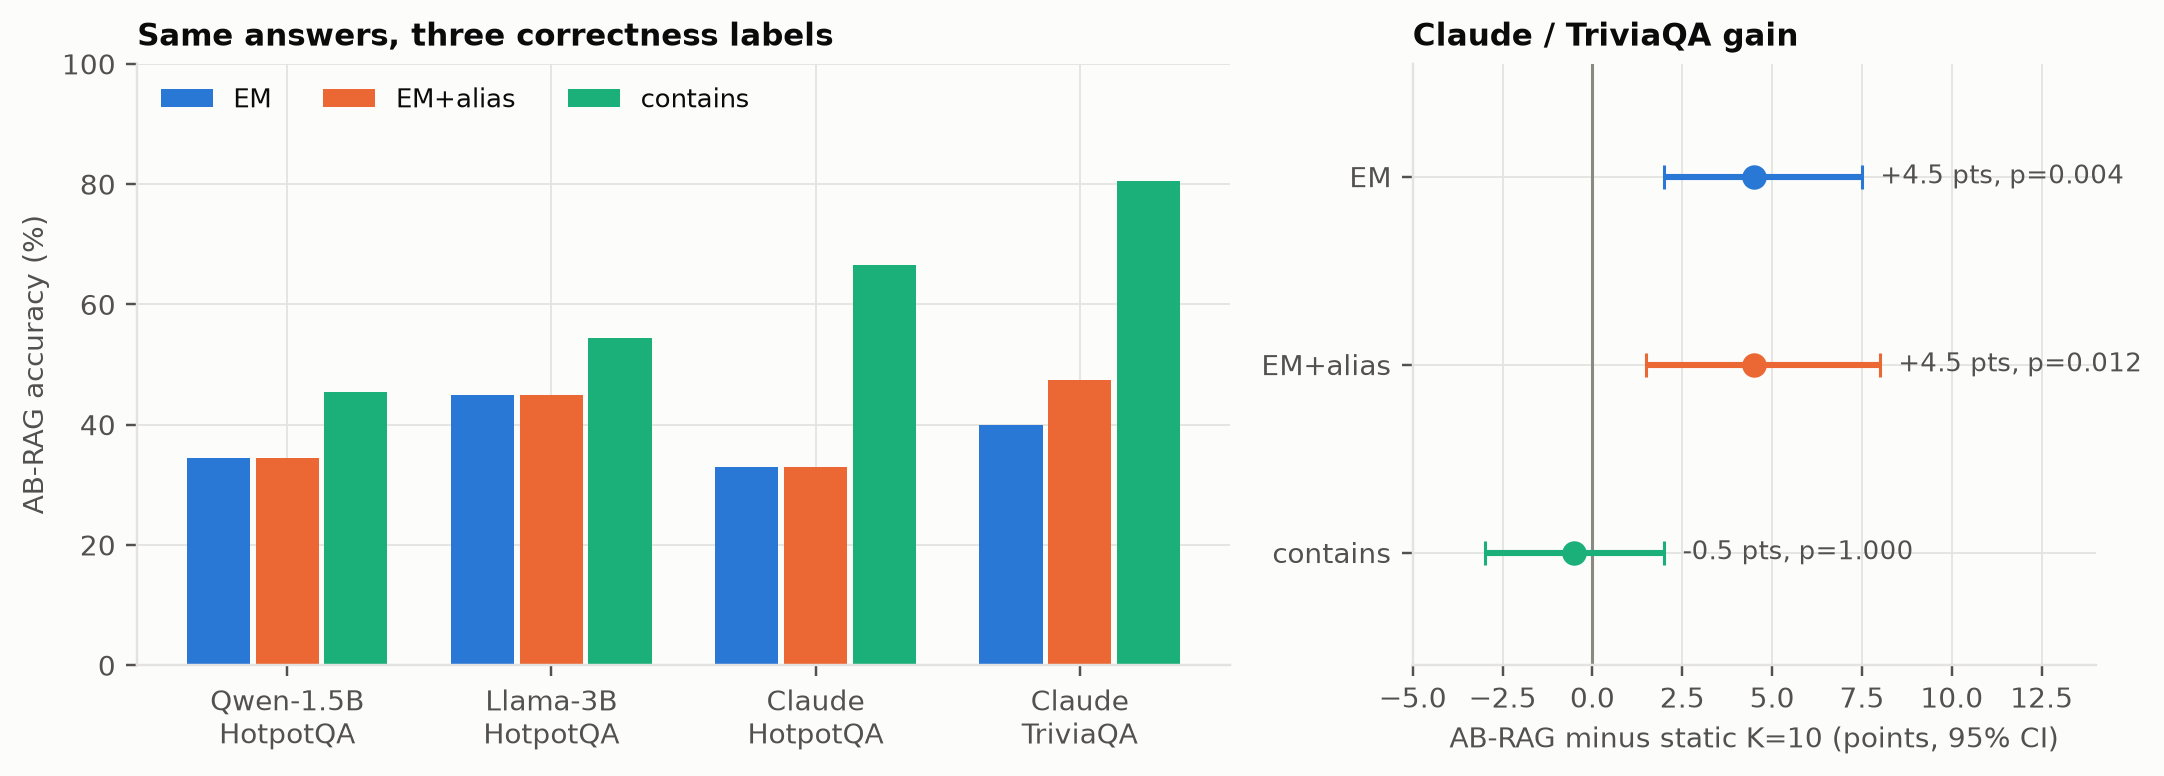
\includegraphics[width=\linewidth]{figures/fig_a_labels_static_vs_abrag.png}
\caption{Left: AB-RAG accuracy on the same answers under three labels. Right: AB-RAG minus static retrieval on Claude/TriviaQA with 95\% bootstrap intervals; the gain disappears under containment.}
\label{fig:labels}
\end{figure}

\subsection{Two of three confidence signals are inert}
\label{sec:signals}

Table~\ref{tab:auroc} gives each signal's first-round AUROC. $S_1$ carries almost all of the information; $S_2$ is below chance for Claude. To measure whether $S_2$ and $S_3$ matter for the decisions AB-RAG actually makes, we recompute every round's confidence with $S_2$ and $S_3$ fixed at their run means, using the weights each run actually used, and count stop decisions that flip. None flip in three runs; 8 of 218 flip for Qwen (Table~\ref{tab:n2}). Across rounds, the spread of confidence contributed by $S_2 + S_3$ is a third of that contributed by $S_1$ for Qwen and between a seventh and a twenty-eighth for the other runs. In practice AB-RAG is a threshold on $S_1$.

\begin{table}[t]
\centering
\small
\begin{tabular}{lcccc}
\toprule
& \multicolumn{3}{c}{First-round AUROC vs.\ \EM{}} & \\
Run & $S_1$ & $S_2$ & $S_3$ & Brevity \\
\midrule
Qwen-1.5B / HotpotQA & 0.607 & 0.517 & 0.571 & 0.615 \\
Llama-3.2-3B / HotpotQA & 0.651 & 0.568 & 0.550 & 0.506 \\
Claude / HotpotQA & 0.769 & 0.353 & 0.572 & 0.848 \\
Claude / TriviaQA & 0.776 & 0.374 & 0.456 & 0.906 \\
\bottomrule
\end{tabular}
\caption{AUROC of each signal, and of answer brevity, for first-round correctness. $S_3$ is the normalized variance the loop used, scored as a reward.}
\label{tab:auroc}
\end{table}

\begin{table}[t]
\centering
\small
\begin{tabular}{lccc}
\toprule
Run & Weights used & Decisions that flip & SD of conf.\ from $S_2{+}S_3$ / from $S_1$ \\
\midrule
Qwen-1.5B / HotpotQA & 0.5 / 0.4 / $-0.1$ & 8 / 218 & 0.021 / 0.065 \\
Llama-3.2-3B / HotpotQA & 0.7 / 0.05 / 0.25 & 0 / 380 & 0.008 / 0.179 \\
Claude / HotpotQA & 0.5 / 0.4 / $-0.1$ & 0 / 272 & 0.020 / 0.145 \\
Claude / TriviaQA & 0.7 / 0.05 / 0.25 & 0 / 362 & 0.007 / 0.199 \\
\bottomrule
\end{tabular}
\caption{Stop decisions (one per executed round) that change when $S_2$ and $S_3$ are held at their run mean.}
\label{tab:n2}
\end{table}

\subsection{Where the gain comes from}
\label{sec:decomp}

AB-RAG differs from the static baseline in two ways: its first round reads five passages instead of ten, and it may iterate. The released logs store each question's first-round answer, so the gain splits into the two parts exactly (Table~\ref{tab:decomp}). On Claude/TriviaQA under \EM{}, 3.0 of the 4.5 points come from starting at five passages and 1.5 from iterating; under containment, starting smaller costs 1.5 points and iterating recovers 1.0. Llama is the one run where iterating dominates ($+5.0$ under every label). Whether confidence chooses \emph{which} questions to iterate on better than chance requires answers for rounds that were never executed; Section~\ref{sec:fulltrace} provides them.

\begin{table}[t]
\centering
\small
\begin{tabular}{llccccc}
\toprule
Run & Label & Static $K{=}10$ & Round 1 ($K{=}5$) & AB-RAG & Start small & Iterate \\
\midrule
Qwen-1.5B / HotpotQA & \EM{} & 34.5 & 35.5 & 34.5 & $+1.0$ & $-1.0$ \\
Llama-3.2-3B / HotpotQA & \EM{} & 39.5 & 40.0 & 45.0 & $+0.5$ & $+5.0$ \\
Claude / HotpotQA & \EM{} & 32.5 & 31.0 & 33.0 & $-1.5$ & $+2.0$ \\
\multirow{3}{*}{Claude / TriviaQA} & \EM{} & 35.5 & 38.5 & 40.0 & $+3.0$ & $+1.5$ \\
& \EM{}+alias & 43.0 & 45.0 & 47.5 & $+2.0$ & $+2.5$ \\
& Contains & 81.0 & 79.5 & 80.5 & $-1.5$ & $+1.0$ \\
\bottomrule
\end{tabular}
\caption{Decomposition of AB-RAG's gain over static retrieval (accuracy in \%, differences in points).}
\label{tab:decomp}
\end{table}

\section{Improvements}
\label{sec:improve}

\subsection{I1: copy-only answer extraction}
\label{sec:i1}

Since much of the \EM{} error is wording, we add a step after generation that reduces each answer to the phrase that answers the question. A small instruction-tuned model (Qwen2.5-1.5B-Instruct, greedy decoding) receives the question and the answer, never the reference, together with five invented few-shot examples (Appendix~\ref{app:i1}). Three fixed rules keep the step a format change: answers of one or two words pass through unchanged; the extracted phrase may only use words that occur in the original answer, otherwise the original is kept; and the extractor never sees the reference answer or any evidence. Answers that state the information is missing are mapped to ``unknown''.

\emph{Disclosure.} The first version of the instruction asked for ``the shortest phrase'' and cut complete names (``Indianapolis Motor Speedway'' became ``Indianapolis''). We revised the instruction once, after reading these errors on the released questions. The numbers below use the revised version, so they are not a clean held-out test; the frozen version is evaluated on the new test split in Section~\ref{sec:fulltrace}.

\subsection{I2: best-round answer}

AB-RAG returns the answer of the round at which it stops. I2 instead returns the answer of the highest-confidence round among those executed, at no extra cost.

\subsection{Results on the released runs}

Table~\ref{tab:improve} and Figure~\ref{fig:improve} apply I1 and I2 to the released answers. I1 never turned an \EM{}-correct answer wrong (0 of 305 across runs) and fixed 8, 2, 25 and 11 answers. I2 matters only for Llama ($+3.0$), the run that iterates most (1.90 rounds on average). The gains are significant for Qwen and both Claude runs (paired bootstrap 95\% intervals $[+1.5, +7.0]$, $[+8.0, +17.0]$ and $[+3.5, +10.0]$ points); Llama's is not under McNemar's test ($p=0.07$, interval $[+0.5, +6.0]$).

\begin{table}[t]
\centering
\small
\begin{tabular}{llcccc}
\toprule
Run & Metric & Paper & + I1 & + I1 + I2 & Paired (I1+I2 vs.\ paper) \\
\midrule
\multirow{3}{*}{Qwen-1.5B / HotpotQA} & \EM{} & 34.5 & 38.5 & 38.5 & $+8/-0$, $p=0.008$ \\
& F1 & 46.2 & 48.7 & 48.7 & \\
& Contains & 45.5 & 44.0 & 44.0 & \\
\midrule
\multirow{3}{*}{Llama-3.2-3B / HotpotQA} & \EM{} & 45.0 & 46.0 & 48.0 & $+7/-1$, $p=0.07$ \\
& F1 & 58.3 & 58.0 & 58.8 & \\
& Contains & 54.5 & 52.5 & 52.5 & \\
\midrule
\multirow{3}{*}{Claude / HotpotQA} & \EM{} & 33.0 & 45.5 & 45.5 & $+25/-0$, $p<0.001$ \\
& F1 & 50.7 & 60.2 & 60.2 & \\
& Contains & 66.5 & 59.0 & 58.0 & \\
\midrule
\multirow{4}{*}{Claude / TriviaQA} & \EM{} & 40.0 & 45.5 & 46.5 & $+13/-0$, $p<0.001$ \\
& \EM{}+alias & 47.5 & 53.5 & 54.5 & $+15/-1$, $p<0.001$ \\
& F1 & 53.5 & 56.5 & 57.5 & \\
& Contains & 80.5 & 70.5 & 71.0 & \\
\bottomrule
\end{tabular}
\caption{I1 and I2 on the released answers (accuracy in \%). Containment falls because I1 turns answers that say the information is missing, but mention the reference in their explanation, into ``unknown'', and cuts the reference away in 3--4 answers per run.}
\label{tab:improve}
\end{table}

These gains change wording, not knowledge: containment does not rise. Two further results follow. First, when static retrieval receives the same extraction step, its Claude/TriviaQA \EM{} rises from 35.5 to 42.5, and AB-RAG's advantage shrinks to $+9/-3$ ($p=0.15$, 95\% CI $[0.0, +6.5]$); under \EM{}+alias it is $+10/-7$ ($p=0.63$). Second, the confidence AUROC under \EM{} falls once answers are short, from 0.682 to 0.639 (Claude/HotpotQA) and from 0.733 to 0.673 (Claude/TriviaQA), and from 0.644 to 0.626 for Llama, while Qwen's rises from 0.600 to 0.619. Part of the published AUROC therefore measured answer length.

\begin{figure}[t]
\centering
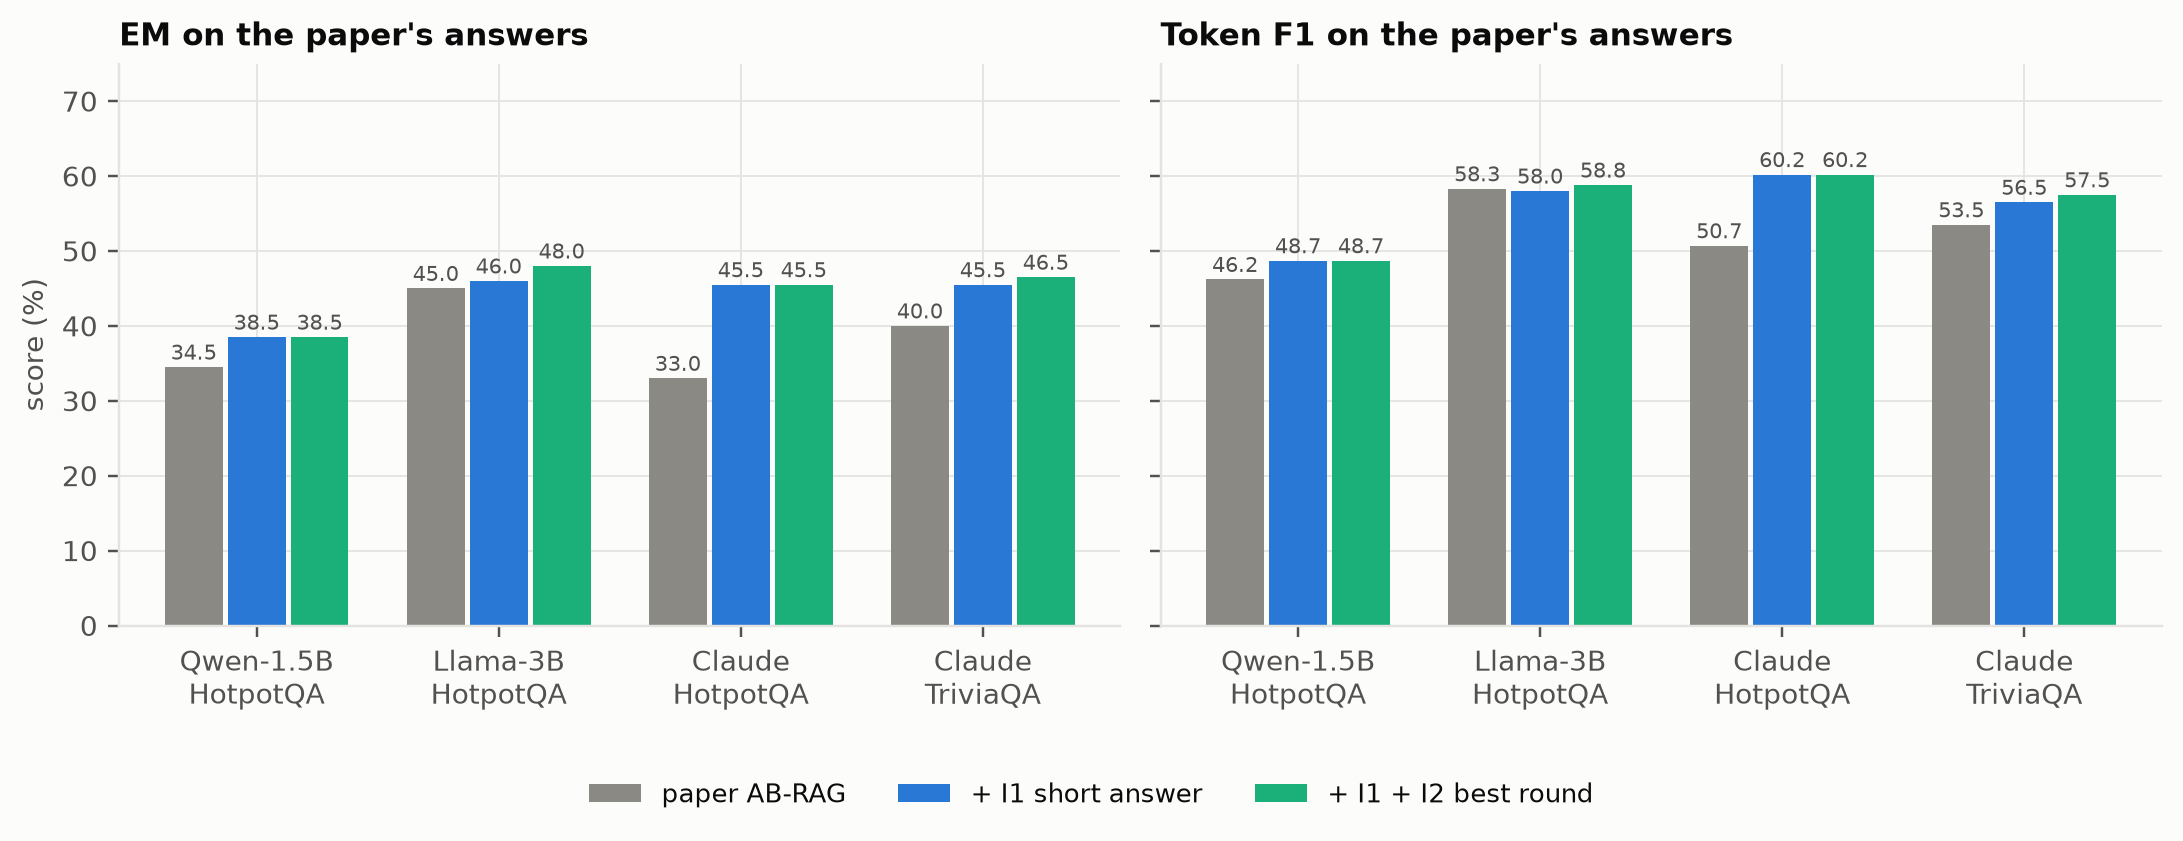
\includegraphics[width=\linewidth]{figures/fig_k_answer_improvements.png}
\caption{\EM{} and F1 on the released answers: as published, with I1, and with I1 + I2.}
\label{fig:improve}
\end{figure}

\subsection{R1: rerank pool and reranker}
\label{sec:r1}

AB-RAG reranks at most 40 passages (the fused top 20 of each retriever), so its reranked recall at 50 cannot exceed the fused list, and at five passages the reranker trails dense retrieval alone (86.6 vs.\ 89.2 recall@5 on HotpotQA). R1 varies two choices: the rerank pool, either the paper's (\emph{rrf20}) or the union of the BM25 and dense top 100 (\emph{union100}), and the cross-encoder, either the paper's MiniLM, bge-reranker-base or bge-reranker-large \citep{xiao2023cpack}. The pair with the best mean recall@5 and @10, the evidence sizes of AB-RAG's first two rounds, on the 300 development questions is reported once on the paper's benchmark setting (Table~\ref{tab:r1}, Figure~\ref{fig:r1}).

On HotpotQA, development questions select the paper's pool with bge-reranker-base (development recall@5 87.2 $\to$ 94.3). On the paper's setting it raises recall@5 from 86.6 to 92.9 and recall@10 from 94.0 to 96.4, and now beats dense retrieval alone at every $k \le 20$. bge-reranker-large scores slightly higher on the paper's setting (93.9 / 96.6) but lost on development questions, and we keep the development choice. On TriviaQA both BGE rerankers lose recall: the better of them reaches 56.5 recall@5 on development questions against MiniLM's 64.0. TriviaQA's gold passages are the chunks that contain an answer string, a distant label, which a reranker that prefers topical passages without the literal answer is penalized under; we did not test whether this explains the drop. The selected TriviaQA configuration keeps MiniLM on the wider pool and stays within 0.4 points of the paper's pipeline at $k \le 10$, so R1 leaves TriviaQA retrieval effectively unchanged, and we run R1 traces on HotpotQA only. The wider pool raises recall@50 (90.8 $\to$ 93.7 on TriviaQA) but not recall at the 5 to 15 passages that AB-RAG reads.

\begin{table}[t]
\centering
\small
\caption{Recall@$k$ (\%) on the paper's setting (HotpotQA first 500 questions, TriviaQA first 200). R1 is the (pool, reranker) pair with the best mean recall@5/@10 on development questions. All rows come from one harness that runs every cross-encoder in half precision; there the paper's pipeline differs from the published values by at most 0.2 points.}
\label{tab:r1}
\begin{tabular}{llccccc}
\toprule
Dataset & Retrieval & @5 & @10 & @15 & @20 & @50 \\
\midrule
\multirow{5}{*}{HotpotQA} & Paper pipeline (rrf20 + MiniLM) & 86.6 & 94.0 & 96.7 & 97.3 & 97.6 \\
& Dense only & 89.2 & 95.3 & 96.9 & 97.2 & 98.3 \\
& union100 + MiniLM & 86.2 & 93.6 & 96.4 & 97.7 & 98.9 \\
& rrf20 + bge-reranker-large & 93.9 & 96.6 & 96.9 & 97.5 & 97.6 \\
& \textbf{R1: rrf20 + bge-reranker-base} & \textbf{92.9} & \textbf{96.4} & 97.3 & 97.6 & 97.6 \\
\midrule
\multirow{4}{*}{TriviaQA} & Paper pipeline (rrf20 + MiniLM) & 67.2 & 80.3 & 85.9 & 88.5 & 90.8 \\
& Dense only & 66.9 & 80.6 & 86.6 & 89.1 & 95.3 \\
& rrf20 + bge-reranker-base & 59.4 & 74.2 & 81.0 & 86.7 & 90.8 \\
& \textbf{R1: union100 + MiniLM} & \textbf{66.9} & \textbf{79.9} & 84.8 & 87.2 & 93.7 \\
\bottomrule
\end{tabular}
\end{table}

\begin{figure}[t]
\centering
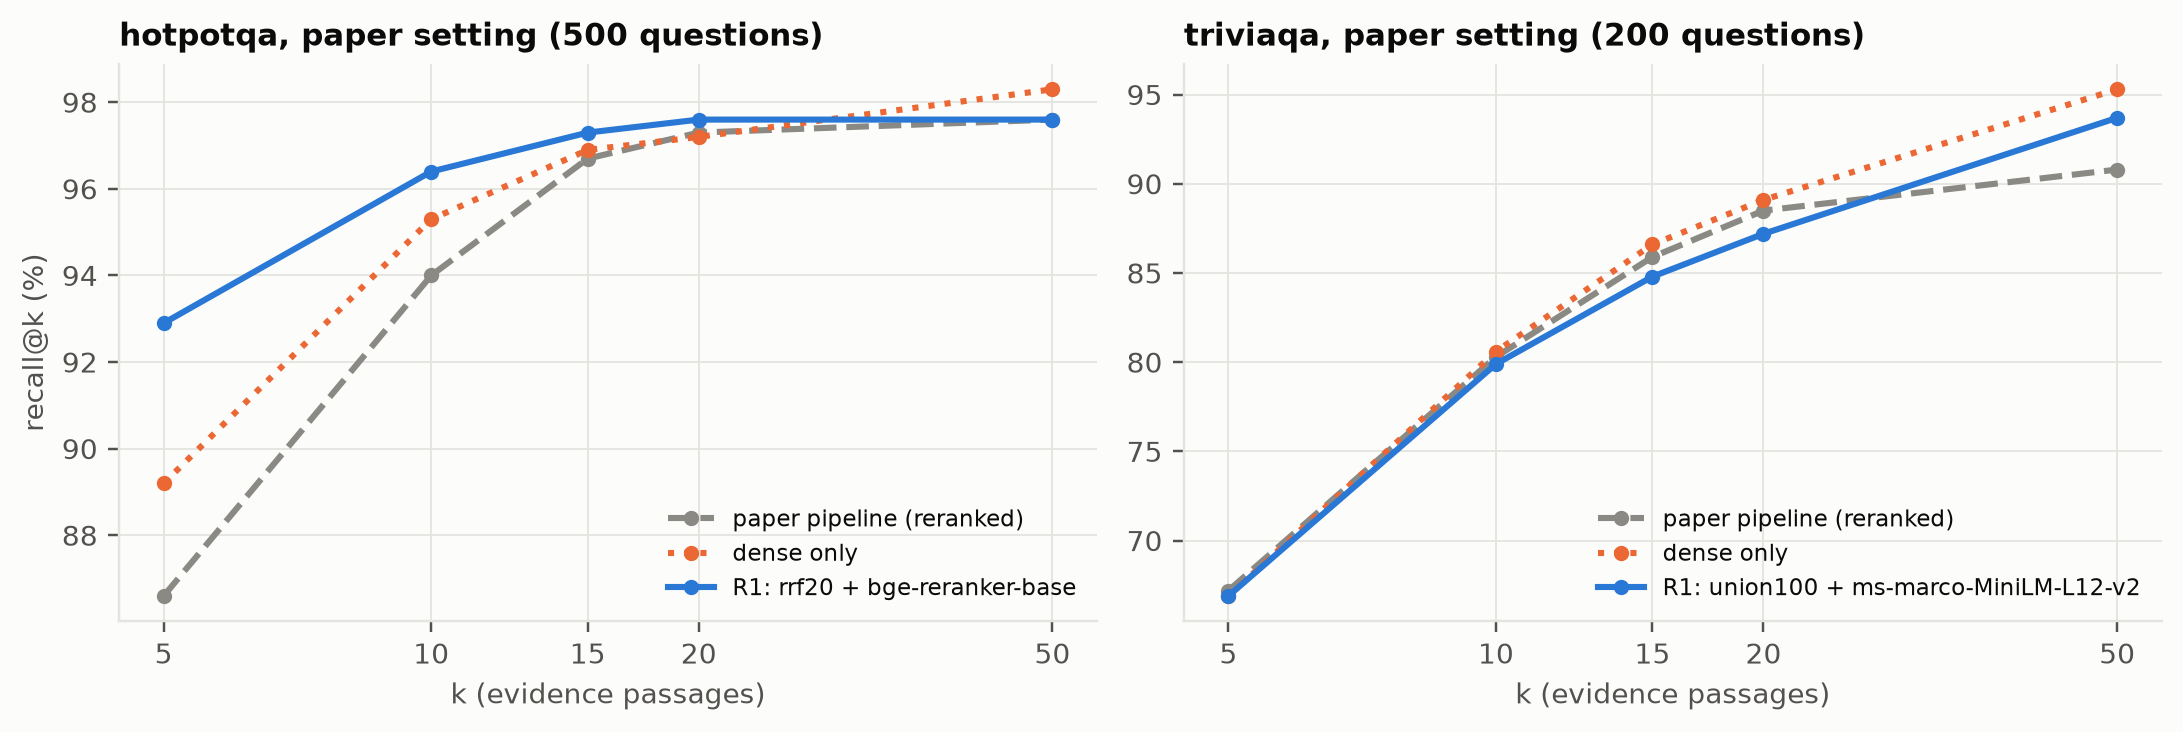
\includegraphics[width=\linewidth]{figures/fig_l_retrieval_upgrade.png}
\caption{Recall@$k$ on the paper's setting: the paper's pipeline, dense retrieval alone, and the R1 configuration chosen on development questions.}
\label{fig:r1}
\end{figure}

\section{Full-trace protocol}
\label{sec:fulltrace}

The released logs contain only the rounds that AB-RAG executed, which limits what can be tested: thresholds above 0.6 cannot be replayed, and a stopping rule cannot be compared with chance. We therefore answer every test question at every round ($K = 5, 10, 15$), with five sampled answers per round, and store all signals. Any stopping rule can then be replayed offline on identical answers: static retrieval at each $K$, AB-RAG at any $\tau$, AB-RAG with I2, an oracle that is correct if any round is correct, and a \textbf{budget-matched random control} that shuffles AB-RAG's stopping rounds across questions (2{,}000 permutations). The random control spends exactly AB-RAG's retrieval budget but ignores confidence, so AB-RAG beats it only if confidence picks the right questions to iterate on. The retrieval corpus pools the passages of all 800 questions (7,947 for HotpotQA and 11,124 for TriviaQA, against 4,963 and 2,582 in the paper), which makes retrieval harder (Appendix~\ref{app:recall}).

\subsection{Results on the new test split}

We regenerate the paper's local configuration, Qwen2.5-1.5B-Instruct with the paper's weights, $\tau = 0.6$ and $K = 5, 10, 15$, on the 500 test questions of each dataset: HotpotQA with the paper's retrieval and with R1, and TriviaQA with the paper's retrieval, since R1 leaves TriviaQA retrieval unchanged (Section~\ref{sec:r1}). I1 is applied to every round's answer with its instruction frozen. On the paper's 200 HotpotQA questions the regenerated pipeline scores 34.0 \EM{} with static retrieval and 36.0 with AB-RAG, against the published 34.5 and 34.5 on a smaller corpus. Table~\ref{tab:fulltrace} gives every stopping rule under \EM{} and containment. \EM{}+alias differs from \EM{} only on TriviaQA and gives the same picture there (AB-RAG 55.8, random stopping 55.6 [54.6, 56.6]).

\begin{table}[t]
\centering
\footnotesize
\setlength{\tabcolsep}{4.5pt}
\begin{tabular}{llcccccccc}
\toprule
Dataset & Pipeline & $K{=}5$ & $K{=}10$ & $K{=}15$ & AB-RAG & Passages & Random [95\% int.] & $P$ & Oracle \\
\midrule
\multicolumn{10}{l}{\emph{\EM{}}} \\
\multirow{4}{*}{HotpotQA} & paper retrieval & 38.0 & 36.2 & 37.6 & 38.0 & 7.4 & 37.9 [37.0, 38.8] & 0.50 & 45.4 \\
& paper + I1 & 41.2 & 40.6 & 42.6 & 42.2 & 7.4 & 41.3 [40.4, 42.4] & 0.06 & 49.8 \\
& R1 & 40.0 & 40.6 & 40.6 & 38.8 & 6.8 & 40.0 [39.2, 41.0] & 1.00 & 48.8 \\
& R1 + I1 & 44.2 & 44.8 & 45.0 & 44.2 & 6.8 & 44.3 [43.4, 45.2] & 0.65 & 52.0 \\
\multirow{2}{*}{TriviaQA} & paper retrieval & 47.8 & 47.4 & 48.8 & 47.8 & 8.1 & 47.9 [46.8, 49.0] & 0.65 & 55.0 \\
& paper + I1 & 50.2 & 50.2 & 51.0 & 50.0 & 8.1 & 50.3 [49.2, 51.2] & 0.78 & 57.4 \\
\midrule
\multicolumn{10}{l}{\emph{Containment}} \\
\multirow{4}{*}{HotpotQA} & paper retrieval & 48.8 & 49.6 & 50.0 & 50.0 & 7.4 & 48.9 [47.8, 50.0] & 0.03 & 58.4 \\
& paper + I1 & 47.8 & 48.6 & 48.8 & 49.0 & 7.4 & 47.9 [46.8, 49.0] & 0.04 & 57.8 \\
& R1 & 51.2 & 52.2 & 52.8 & 51.4 & 6.8 & 51.3 [50.4, 52.2] & 0.52 & 59.6 \\
& R1 + I1 & 50.2 & 51.2 & 51.2 & 50.4 & 6.8 & 50.3 [49.4, 51.2] & 0.49 & 58.0 \\
\multirow{2}{*}{TriviaQA} & paper retrieval & 66.6 & 67.2 & 66.6 & 67.0 & 8.1 & 66.6 [65.6, 67.6] & 0.32 & 74.0 \\
& paper + I1 & 66.4 & 66.4 & 65.6 & 66.8 & 8.1 & 66.3 [65.2, 67.4] & 0.25 & 73.4 \\
\bottomrule
\end{tabular}
\caption{Full traces on the 500 test questions per dataset (Qwen2.5-1.5B-Instruct, accuracy in \%). Static $K$ answers once from $K$ passages; AB-RAG stops at $\tau = 0.6$ and reads the mean number of passages shown (static $K$ reads $K$). Random stopping shuffles AB-RAG's stopping rounds across questions, so it reads the same passages; $P$ is the share of its 2{,}000 permutations at least as accurate as AB-RAG. Oracle counts a question as correct if any round answers it correctly.}
\label{tab:fulltrace}
\end{table}

\paragraph{Confidence-based stopping is no better than random stopping.} At $\tau = 0.6$, AB-RAG's \EM{} lies inside the 95\% interval of the random control in five of six pipelines and below it in the sixth (R1: 38.8 against 40.0 [39.2, 41.0]). Figure~\ref{fig:ftsweep} repeats the comparison at every threshold from 0.30 to 0.95 with 1{,}000 permutations each. Of the 100 combinations of pipeline, label and threshold at which AB-RAG and the control can differ, AB-RAG lies above the control's interval in eight, by at most 0.6 points and seven of them under containment, and below it in three, all under \EM{} with R1. AB-RAG never differs significantly from static $K=10$ (all $p > 0.18$), while reading 6.8 to 8.1 passages instead of 10. The stopping rounds explain why: confidence passes $\tau$ after the first round for 85 to 91\% of questions, so AB-RAG behaves almost like static retrieval with five passages, and with the paper's retrieval it has exactly the \EM{} of static $K=5$ on both datasets. More evidence barely helps this model, as static $K=5$ and $K=15$ differ by at most 1.4 points \EM{} in every pipeline. Yet for 7 to 10 points of questions some round does answer correctly (the oracle), so a stopping rule has room to gain; the confidence score does not find it.

\begin{figure}[t]
\centering
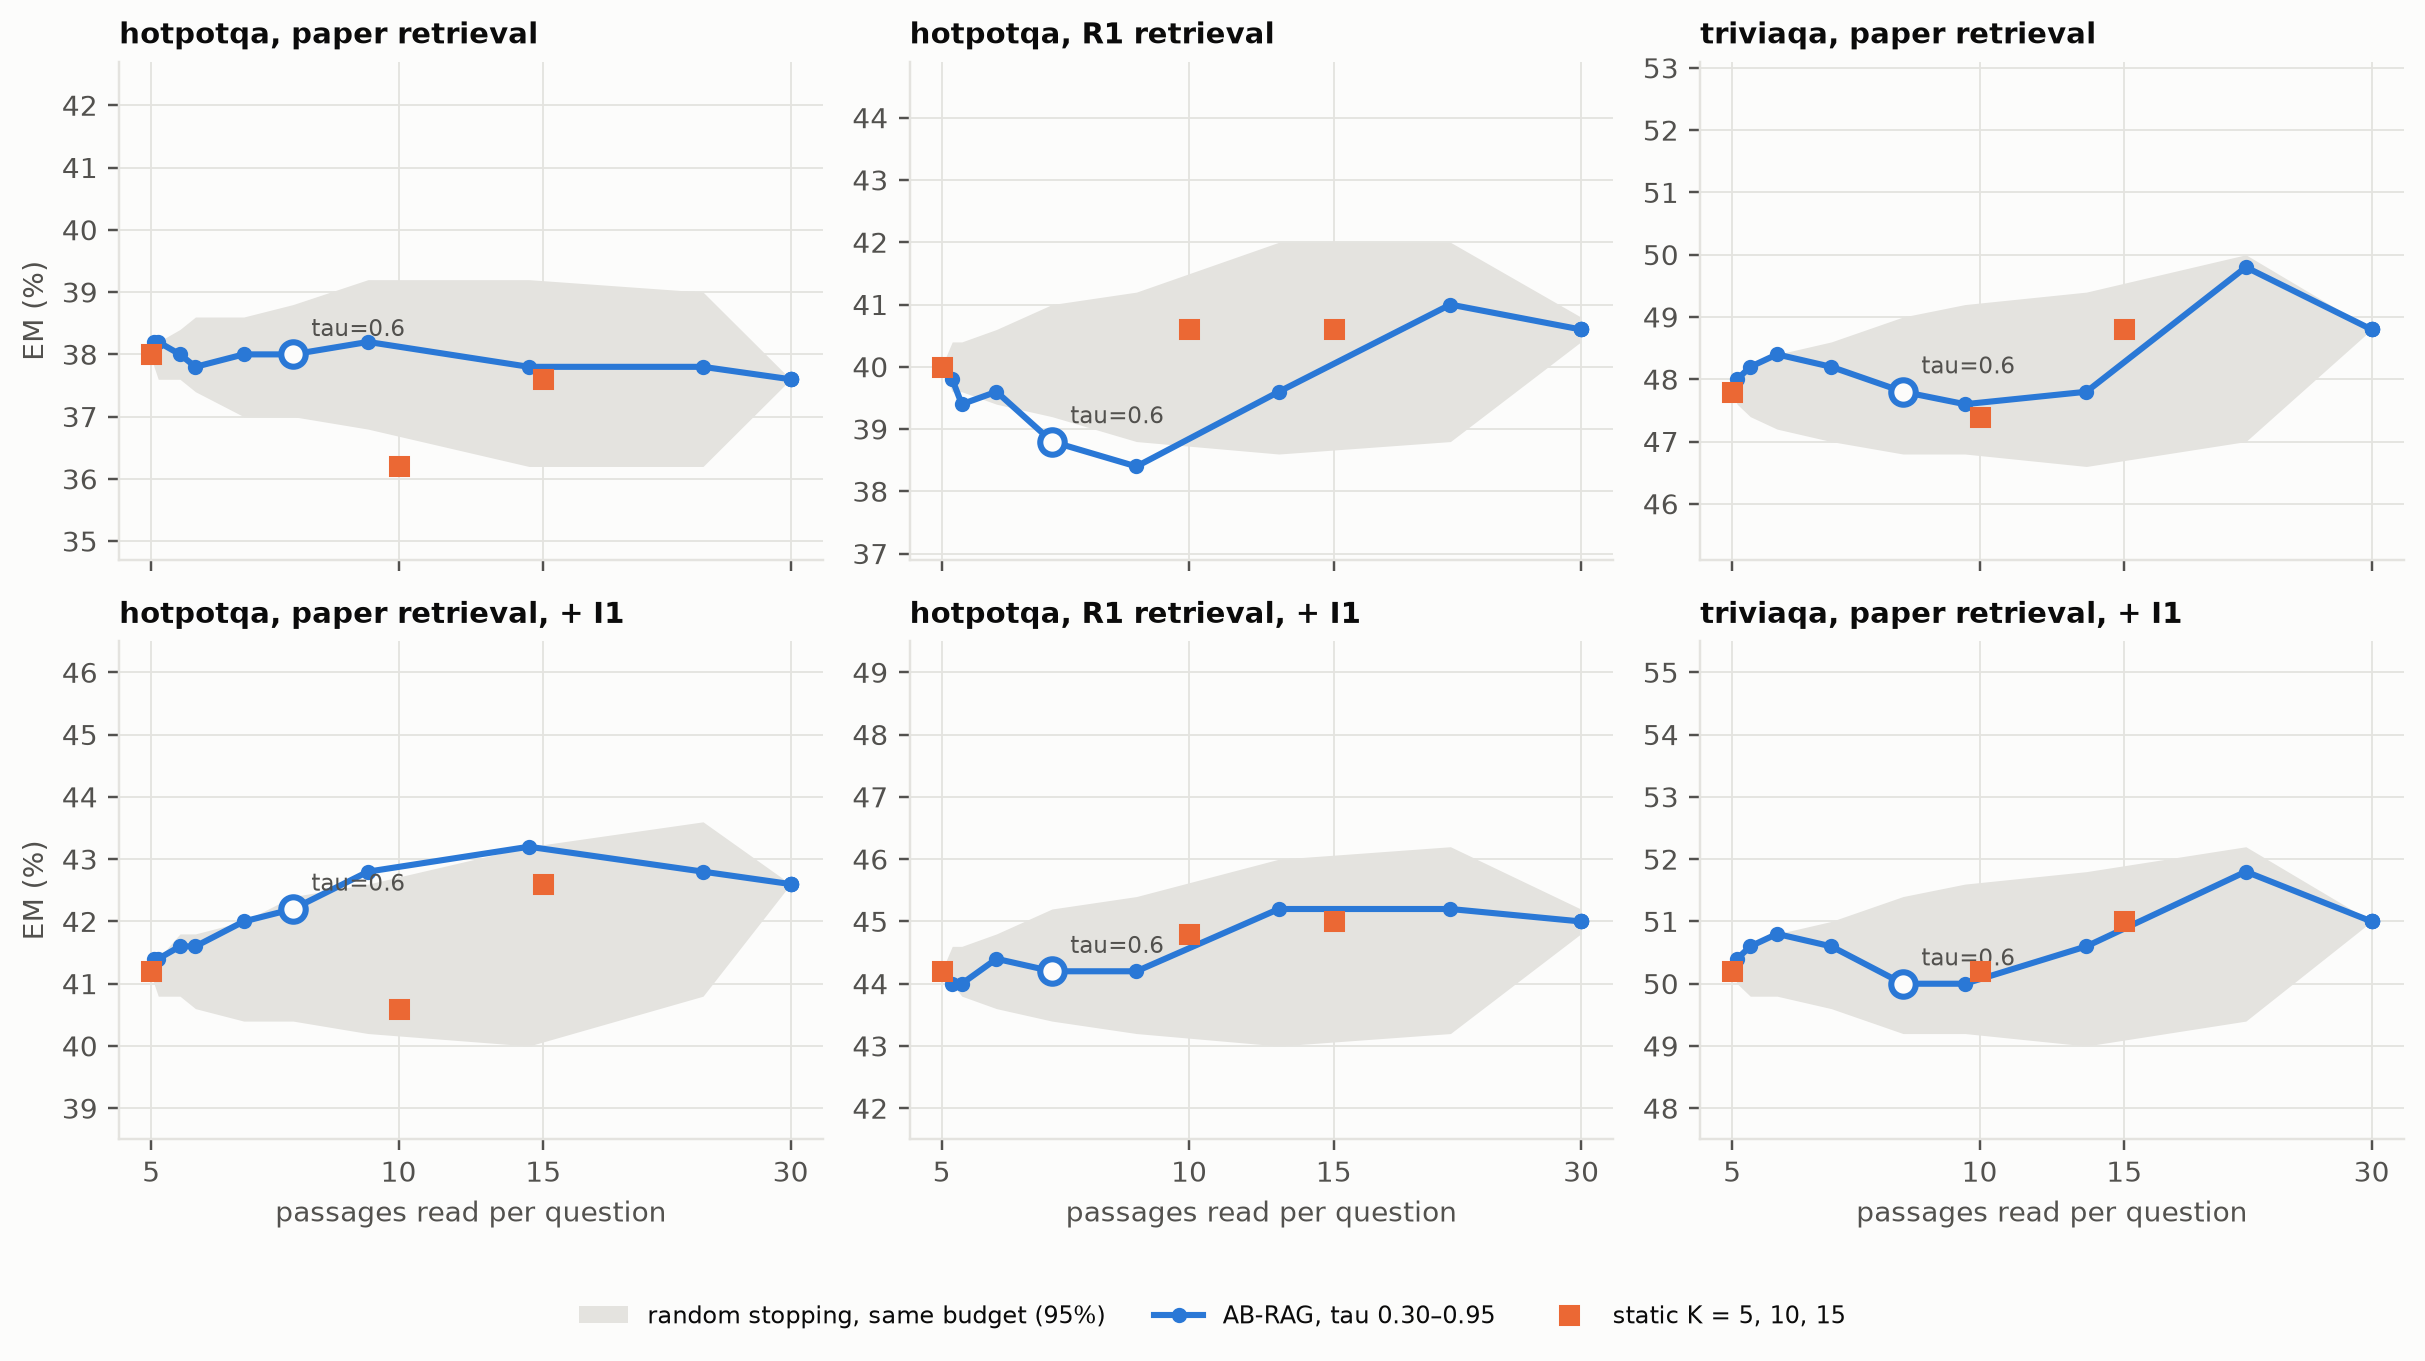
\includegraphics[width=\linewidth]{figures/fig_m_fulltrace_tau_sweep.png}
\caption{\EM{} against mean passages read on the 500 test questions. Line: AB-RAG at $\tau$ from 0.30 to 0.95 (open circle at $\tau = 0.6$). Band: 95\% interval of random stopping with the same budget at each $\tau$; it closes where every question stops at the same round. Squares: static $K = 5, 10, 15$. Top row: answers as generated; bottom row: with I1.}
\label{fig:ftsweep}
\end{figure}

\paragraph{N2 and N3 replicate.} Holding $S_2$ and $S_3$ at their run mean flips 3 of 602, 8 of 576 and 3 of 627 executed stop decisions (HotpotQA with the paper's retrieval, with R1, and TriviaQA). Across rounds, $S_2$ and $S_3$ together contribute a standard deviation of 0.008 to 0.010 to the confidence score, against 0.073 to 0.082 from $S_1$, and the first-round AUROC of the confidence score is within 0.01 of that of $S_1$ alone (0.648 vs.\ 0.652 on HotpotQA, 0.770 vs.\ 0.770 on TriviaQA). Answer brevity predicts \EM{}-correctness (AUROC 0.61 on both datasets) but not containment-correctness (0.46 and 0.43), as on the released Qwen run (0.62 and 0.49); on the released Claude runs brevity also predicts containment-correctness (0.63 and 0.80).

\begin{table}[t]
\centering
\footnotesize
\setlength{\tabcolsep}{4.5pt}
\begin{tabular}{llccccc}
\toprule
Dataset & Change & Accuracy & $+/-$ & $p$ & 95\% CI (pts) & Questions 201--500: $\Delta$ ($p$) \\
\midrule
\multicolumn{7}{l}{\emph{\EM{}}} \\
HotpotQA & I1 & 38.0 $\to$ 42.2 & $+21/-0$ & $<$0.001 & [$+$2.4, $+$6.0] & $+$4.7 ($<$0.001) \\
TriviaQA & I1 & 47.8 $\to$ 50.0 & $+11/-0$ & $<$0.001 & [$+$1.0, $+$3.6] & $+$2.4 (0.016) \\
HotpotQA & I2 & 38.0 $\to$ 38.0 & $+1/-1$ & 1.00 & [$-$0.6, $+$0.6] & $+$0.4 (1.00) \\
TriviaQA & I2 & 47.8 $\to$ 47.6 & $+0/-1$ & 1.00 & [$-$0.6, $+$0.0] & $-$0.3 (1.00) \\
HotpotQA & R1, static $K{=}10$ & 36.2 $\to$ 40.6 & $+44/-22$ & 0.009 & [$+$1.2, $+$7.6] & $+$4.3 (0.053) \\
HotpotQA & R1, AB-RAG & 38.0 $\to$ 38.8 & $+36/-32$ & 0.72 & [$-$2.4, $+$4.0] & $+$0.7 (0.87) \\
HotpotQA & R1 + I1, static $K{=}10$ & 36.2 $\to$ 44.8 & $+62/-19$ & $<$0.001 & [$+$5.2, $+$12.2] & $+$8.3 ($<$0.001) \\
HotpotQA & R1 + I1, AB-RAG & 38.0 $\to$ 44.2 & $+56/-25$ & $<$0.001 & [$+$2.8, $+$9.8] & $+$6.0 (0.013) \\
\midrule
\multicolumn{7}{l}{\emph{Containment}} \\
HotpotQA & I1 & 50.0 $\to$ 49.0 & $+0/-5$ & 0.06 & [$-$2.0, $-$0.2] & $-$0.3 (1.00) \\
TriviaQA & I1 & 67.0 $\to$ 66.8 & $+0/-1$ & 1.00 & [$-$0.6, $+$0.0] & $-$0.4 (1.00) \\
HotpotQA & R1, static $K{=}10$ & 49.6 $\to$ 52.2 & $+45/-32$ & 0.17 & [$-$0.8, $+$6.0] & $+$2.7 (0.30) \\
HotpotQA & R1, AB-RAG & 50.0 $\to$ 51.4 & $+46/-39$ & 0.52 & [$-$2.2, $+$5.0] & $+$0.7 (0.89) \\
HotpotQA & R1 + I1, static $K{=}10$ & 49.6 $\to$ 51.2 & $+44/-36$ & 0.43 & [$-$2.0, $+$5.2] & $+$1.7 (0.56) \\
HotpotQA & R1 + I1, AB-RAG & 50.0 $\to$ 50.4 & $+46/-44$ & 0.92 & [$-$3.4, $+$4.2] & $+$0.3 (1.00) \\
\bottomrule
\end{tabular}
\caption{Each change against the base pipeline (the paper's retrieval, answers as generated) under the same stopping policy, paired question by question on the 500 test questions: questions gained and lost, McNemar exact $p$, and a paired bootstrap 95\% interval. The last column repeats the comparison on questions 201--500, which are outside the paper's runs and played no part in revising I1. Under containment I2 changes two labels per dataset (HotpotQA $+1/-1$, TriviaQA $+2/-0$, $p \ge 0.50$).}
\label{tab:ftpaired}
\end{table}

\paragraph{I1 holds on unseen questions; I2 has nothing to select.} Table~\ref{tab:ftpaired} pairs each change with the base pipeline question by question. I1 raises \EM{} by 4.2 points on HotpotQA and 2.2 on TriviaQA without turning a single \EM{}-correct answer wrong, and the gain holds on questions 201--500, which played no part in revising its instruction ($+4.7$, $p<0.001$, and $+2.4$, $p=0.016$). Containment falls by 1.0 and 0.2 points. I2 changes the \EM{} label of at most two answers per dataset: with 1.2 rounds on average there is rarely an earlier, more confident round to return. With I1 and I2 together AB-RAG scores 42.0 and 49.8 \EM{}, against 42.2 and 50.0 with I1 alone.

\paragraph{R1 helps static retrieval but not AB-RAG.} The stronger reranker raises static $K=10$ \EM{} on HotpotQA from 36.2 to 40.6 ($p=0.009$; $+4.3$ on questions 201--500, $p=0.053$) and containment by 2.6 points ($p=0.17$). AB-RAG gains only 0.8 points ($p=0.72$): R1 raises first-round \EM{} by 2.0 points, but the few questions AB-RAG sends to further rounds then lose more answers than they gain ($-1.2$ points against stopping after the first round). With R1 and I1 together, AB-RAG reaches 44.2 \EM{} ($+6.2$ over the base pipeline, $p<0.001$; $+6.0$ on questions 201--500, $p=0.013$), and static $K=10$ with the same two changes reaches 44.8 ($+8.6$ over static $K=10$ with the paper's retrieval). On top of I1, R1 alone still adds 4.2 points to static $K=10$ ($40.6 \to 44.8$, $+46/-25$, $p=0.017$; $+4.3$ on questions 201--500, $p=0.072$). Neither combination raises containment significantly, so most of the \EM{} gain is again answer format, with a smaller part from retrieval.

\section{Discussion}

The released runs support AB-RAG's \EM{} numbers but not the reading that adaptive retrieval makes answers more often correct. On the one run where the comparison can be paired, the advantage over static retrieval is tied to wording and disappears under a wording-independent label or when both systems receive the same extraction step. Confidence AUROC under \EM{} partly reflects answer length, and the confidence score is in effect a threshold on one signal. The full traces test the remaining claim directly: with the paper's open model, choosing which questions to iterate on by confidence is no better than choosing them at random, although the oracle shows that the right round exists for 7 to 10 points of questions. A useful stopping rule would need a signal that separates those questions, which the token-probability signal $S_1$ does not.

For practitioners the results suggest a simple order of work. Fixing the answer format (I1) is cheap and gives the largest \EM{} gain; a stronger reranker (R1) helps every pipeline that reads few passages; and an adaptive stopping rule should be adopted only after it beats random stopping with the same budget on the model it will serve.

\section{Conclusion}

Re-scoring released runs is cheap and revealing. For AB-RAG it confirms the published numbers, locates four inconsistencies, and shows that the reported gains and calibration depend on answer wording more than on retrieval decisions. Simple, transparent post-processing raises exact match by 3 to 12.5 points without making more answers contain the reference, and on 500 new questions per dataset the confidence-based stopping rule matches a random rule with the same budget. Together these argue for reporting a wording-independent label, paired tests, and a budget-matched random control whenever adaptive retrieval is evaluated with exact match.

\section*{Limitations}

Each released run covers 200 questions with one sample of the system, so differences of one or two points are within noise, as the confidence intervals show. Containment is a lenient label and over-credits answers that mention the reference while asserting something else; we report it next to \EM{}, not instead of it. I1 relies on a 1.5B-parameter extractor that sometimes picks the wrong phrase, and its instruction was revised once on the evaluated questions. We did not regenerate the Claude or Llama runs. The full-trace experiments use a single open model of 1.5B parameters, for which more evidence changes \EM{} by at most 1.4 points, so they test AB-RAG where adaptive retrieval has little to gain on average; a larger generator that uses additional passages better could leave a stopping rule more room. R1 was evaluated end to end on HotpotQA only, and we tested three cross-encoders, not the full space of rerankers.

\section*{Reproducibility and ethics statement}

All analyses use the code, data and logs released with AB-RAG under the MIT license, which we cite and credit; we did not reuse its text or figures. Our code recomputes every number in this paper from the saved outputs. No new paid API calls were made. The extraction step runs on a single consumer GPU; the full traces took about 20 minutes on three data-center GPUs, and the released notebook reproduces them on one free cloud GPU in several hours. The datasets are public question-answering benchmarks without personal data.

\bibliographystyle{plainnat}
\bibliography{refs}

\appendix

\section{The I1 extractor}
\label{app:i1}

The instruction reads: \emph{Extract the answer to the question from the response. Copy the exact words of the phrase that answers the question and keep names and titles complete. Remove only explanations, extra sentences and lead-ins. For a yes/no question write yes or no. If the response is already just the answer, copy it unchanged. If the response says the information is unknown or missing, write: unknown.} Five few-shot examples with invented names follow (a stadium name inside a sentence, a yes/no answer, an author name, an answer that is already short, and an ``unknown'' answer), so that no evaluated question or answer appears in the prompt. Examples of its effect on the released Claude/HotpotQA answers:

\begin{center}
\small
\begin{tabular}{lll}
\toprule
Reference & Original answer & After I1 \\
\midrule
yes & Yes, both American. & yes \\
Terry Richardson & Terry Richardson is older. (Annie Morton was born \ldots) & Terry Richardson \\
3,677 seated & 4,000 capacity (3,677 seated) & 3,677 \\
Chief of Protocol & Unknown. The evidence identifies Shirley Temple as \ldots & unknown \\
\bottomrule
\end{tabular}
\end{center}

\section{Threshold sweep}
\label{app:sweep}

\begin{center}
\small
\begin{tabular}{lcccc}
\toprule
& & \multicolumn{2}{c}{Avg.\ rounds / \EM{}} & \\
Run & $\tau$ & Paper & Replayed from logs & \\
\midrule
Claude / HotpotQA & 0.30 & 1.00 / 32.5 & 1.00 / 31.0 & differs \\
 & 0.45 & 1.14 / 32.5 & 1.00 / 31.0 & differs \\
 & 0.60 & 1.36 / 33.0 & 1.36 / 33.0 & match \\
Claude / TriviaQA & 0.30 & 1.00 / 35.5 & 1.00 / 38.5 & differs \\
 & 0.45 & 1.30 / 37.0 & 1.33 / 40.0 & differs \\
 & 0.60 & 1.81 / 40.0 & 1.81 / 40.0 & match \\
Qwen-1.5B / HotpotQA & 0.30 & 1.00 / 34.5 & 1.00 / 35.5 & differs \\
 & 0.45 & 1.02 / 34.5 & 1.00 / 35.5 & differs \\
 & 0.60 & 1.09 / 34.5 & 1.09 / 34.5 & match \\
\bottomrule
\end{tabular}
\end{center}

\section{Open-retrieval recall}
\label{app:recall}

Recall@$k$ (\%) for $k = 5, 10, 20, 50$. ``Paper setting'' is our rerun of the released benchmark (HotpotQA first 500 questions, TriviaQA first 200); it equals the published values in every cell. The 800-question pool is the corpus of the full-trace runs.

\begin{center}
\small
\begin{tabular}{llcc}
\toprule
Dataset & Method & Paper setting (= published) & 800-question pool \\
\midrule
\multirow{4}{*}{HotpotQA} & BM25 & 58.7 / 72.8 / 80.9 / 86.2 & 59.7 / 72.2 / 79.8 / 85.0 \\
& Dense & 89.2 / 95.3 / 97.2 / 98.3 & 88.8 / 94.0 / 96.2 / 97.9 \\
& Hybrid & 79.8 / 93.3 / 96.9 / 97.6 & 80.0 / 92.5 / 96.2 / 97.2 \\
& Reranked & 86.6 / 94.0 / 97.3 / 97.6 & 86.2 / 93.9 / 96.8 / 97.2 \\
\midrule
\multirow{4}{*}{TriviaQA} & BM25 & 43.6 / 54.1 / 63.7 / 69.6 & 38.4 / 46.7 / 53.4 / 60.6 \\
& Dense & 66.9 / 80.6 / 89.1 / 95.3 & 58.1 / 71.1 / 80.7 / 88.6 \\
& Hybrid & 59.4 / 75.8 / 86.2 / 90.8 & 52.3 / 66.9 / 77.4 / 83.5 \\
& Reranked & 67.0 / 80.3 / 88.4 / 90.8 & 61.4 / 74.1 / 81.3 / 83.5 \\
\bottomrule
\end{tabular}
\end{center}

\end{document}
